\chapter{Results}
\label{chap_results}
\section{Optimised \texorpdfstring{\acrshort{uav}}{UAV} Parameters}
%\hl{DETAIL \& PLOT THE OPTIMISATION CURVES FOR THE VARIOUS PARAMETERS OF THE UAV \& UAV-GU COMMUNICATIONS}
The parameters that were optimised by maximisation and minimisation of values were the \acrshort{uav} energy efficiency $\eta_{EE} (T)$, the data exchange rate $R_{U, k} [n]$ between the \acrshort{uav} and \acrshort{lu}s, the total secrecy rate $R_{U, k}^{sec}$ and the \acrshort{uav} trajectory $c(t)$, leading to a decrease in the distances between the \acrshort{uav}-\acrshort{bs} and \acrshort{lu}s. 
\subsection{\texorpdfstring{\acrshort{uav}}{UAV} Trajectory}
For $\eta_{EE}(t)$, $R_{U, k} (t)$ and $R_{U, k}^{sec}$ to be optimised, the \acrshort{uav} trajectory also had to be optimised to fairly and securely provide coverage to all of the \acrshort{lu}s. 
This involved ensuring that distance to the \acrshort{gu} centroid as well as a smaller difference in distance between the \acrshort{uav} and all of the \acrshort{lu}s were minimised and that rewards were allocated to the agent for minimising these values from timestep to timestep. 

%\begin{figure}[ht!]
%   \centering
%       \subfigure[Maximum, Minimum \& Mean Distances to \acrshort{lu} Centroid Per Timestep Across 30 Episodes]{\label{fig:step_dist_to_centroid}
%           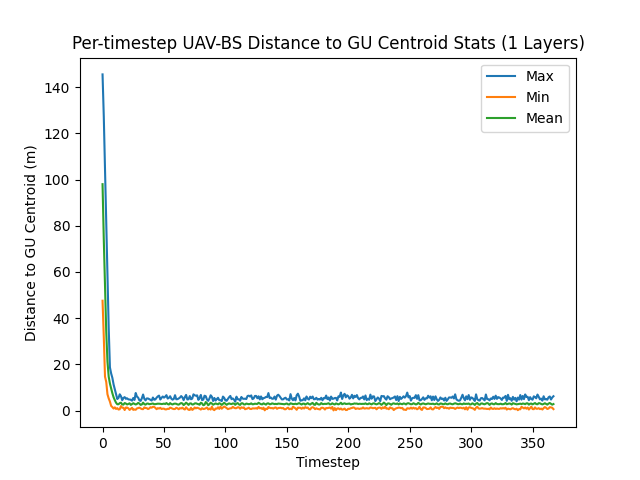
\includegraphics[width=0.43\textwidth]{figures/eve_test1/1_timestep_distance_to_centroid.png}
%       }
%       \hspace{1mm}
%    \subfigure[Maximum, Minimum \& Mean Distances to the \acrshort{lu} Centroid Across 30 Episodes]{\label{fig:ep_dist_to_centroid}
%           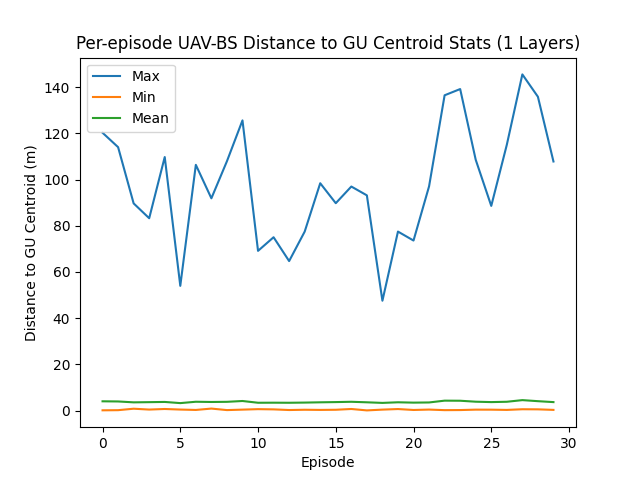
\includegraphics[height=0.21\textheight]{figures/eve_test1/1_episode_distance_to_centroid.png}
%       }
%       \caption{Proximity of the \acrshort{uav} to the \acrshort{lu} Centroid}
%       \label{fig:dist_to_centroid_plots}
%\end{figure}
\begin{figure} [ht!]
    \centering
    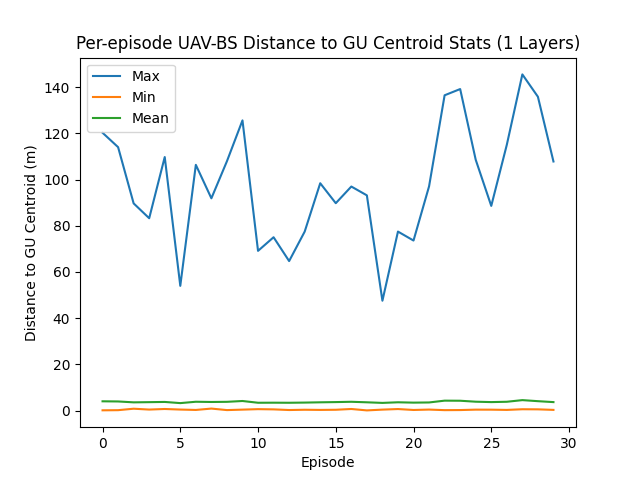
\includegraphics[width=0.75\linewidth]{figures/eve_test1/1_episode_distance_to_centroid.png}
    \caption{Maximum, Minimum \& Mean Distances to the \acrshort{lu} Centroid Across 30 Episodes}
    \label{fig:episode_dist_to_centroid}
\end{figure}
\begin{figure} [ht!]
    \centering
    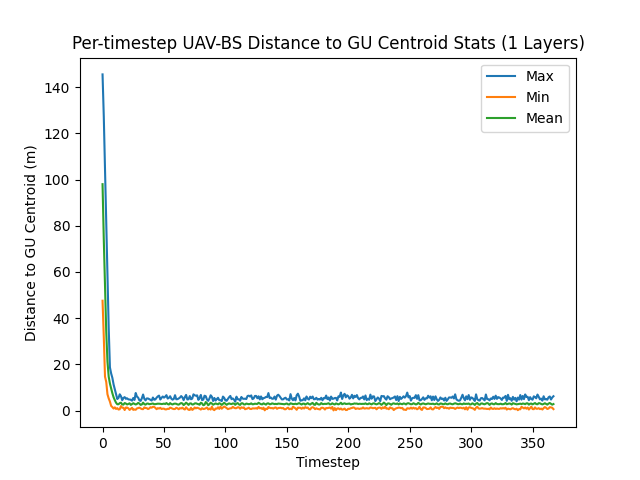
\includegraphics[width=0.75\linewidth]{figures/eve_test1/1_timestep_distance_to_centroid.png}
    \caption{Maximum, Minimum \& Mean Distances to \acrshort{lu} Centroid Per Timestep Across 30 Episodes}
    \label{fig:timestep_dist_to_centroid}
\end{figure}
As can be seen in Fig. \ref{fig:episode_dist_to_centroid} and Fig. \ref{fig:timestep_dist_to_centroid}, the \acrshort{uav} converged towards the \acrshort{lu} centroid (10 m above the average x, y co-ordinates for all \acrshort{lu}s) from a number of randomly generated starting locations where it was initialised in each episode. 
This demonstrates that the \acrshort{uav} consistently learned to achieve this objective, regardless of where it started in the simulation. 

\begin{figure} [ht!]
    \centering
    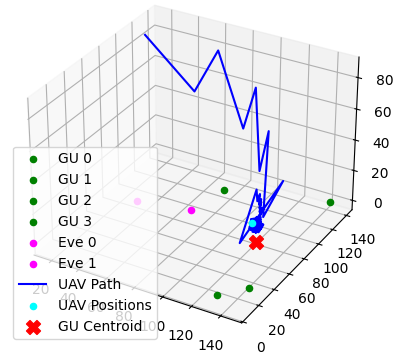
\includegraphics[width=0.75\linewidth]{figures/1_layers_uav_trajectory_20_timestep_370.png}
    \caption{\acrshort{uav} Trajectory in Simulated Environment}
    \label{fig:uav_trajectory_cube}
\end{figure}
As can be seen in Fig. \ref{fig:uav_trajectory_cube}, the \acrshort{uav} managed to learn, based on the observed state of the environment, to converge on the centroid of the \acrshort{lu}s despite its initial position being on the far side of the flight area. 
\subsection{Energy Efficiency}
The stabilisation and convergence of $\eta(t)$, i.e., the energy efficiency at timestep $t$ and $\eta (T)$, i.e., the integral of the energy efficiency from $t=0$ to $t=T$ is shown in Fig. \ref{fig:step_energy_eff} \& \ref{fig:ep_energy_eff}, respectively. 
A mean value of ~40kbps/Hz/J for $\eta(T)$ is maintained for all episodes in the simulation as the agent exhibits that it can and does effectively learn to optimise $\eta(t)$ early in the simulation with a single-layered ansatz in the actor and critic networks' quantum circuits. 
\begin{figure} [ht!]
    \centering
    %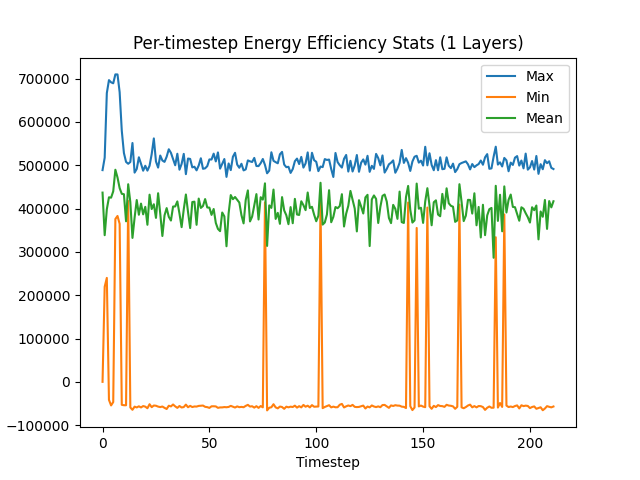
\includegraphics[width=0.75\linewidth]{figures/test9/1_timestep_energy_eff.png}
    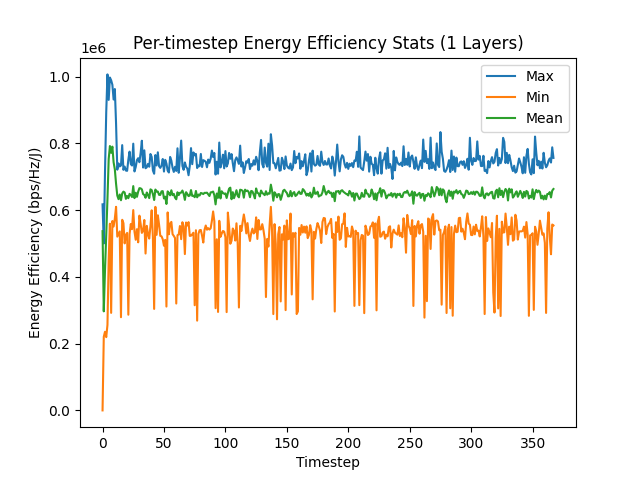
\includegraphics[width=0.75\linewidth]{figures/plots_eve_outputs/test3/1_timestep_energy_eff.png}
    \caption{Maximum, Minimum \& Mean Energy Efficiency Per Timestep}
    \label{fig:step_energy_eff}
\end{figure}

\begin{figure} [ht!]
    \centering
    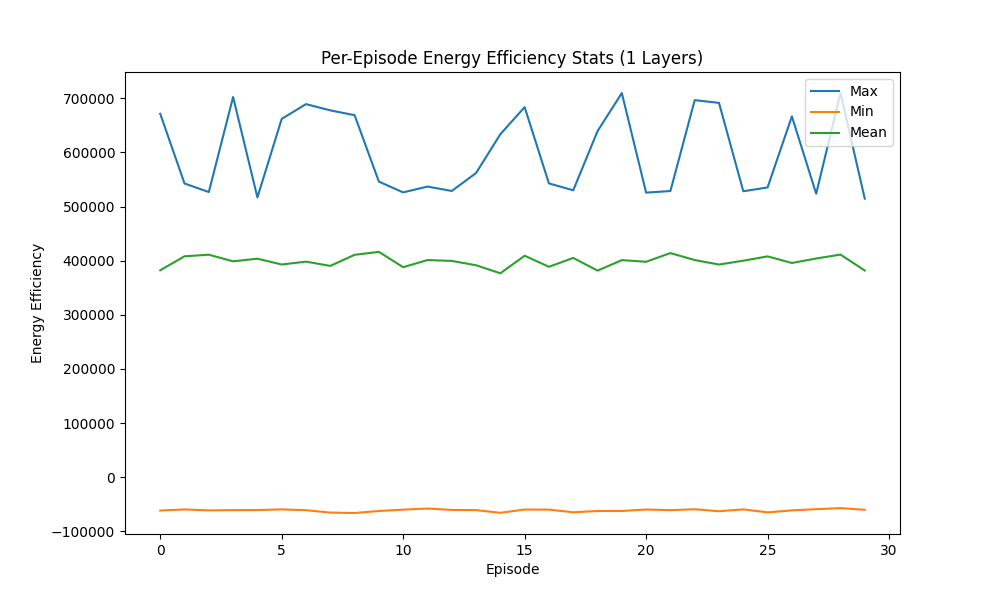
\includegraphics[width=0.75\linewidth]{figures/test9/1_episode_energy_eff.png}
    \caption{Energy Efficiency Across 30 Episodes}
    \label{fig:ep_energy_eff}
\end{figure}
As shown in Fig. \ref{fig:step_energy_eff} and Fig. \ref{fig:ep_energy_eff}, $\eta_{EE} (t)$ converges consistently towards \~ 40kbps/Hz/J across all of the 30 episodes that were run. 

As the \acrshort{uav} trajectory has been optimised as well as the data exchange rate and the secrecy rate, the energy efficiency increases as the \acrshort{uav} converges towards a lower level of energy consumption as it ceases to move around the environment and is able to hover above the optimal location for secure communications with the \acrshort{lu}s. 

%\begin{figure}[ht!]
%   \centering
%       \subfigure[Maximum, Minimum \& Mean Energy Efficiency Per Timestep]{\label{fig:step_energy_eff}
%           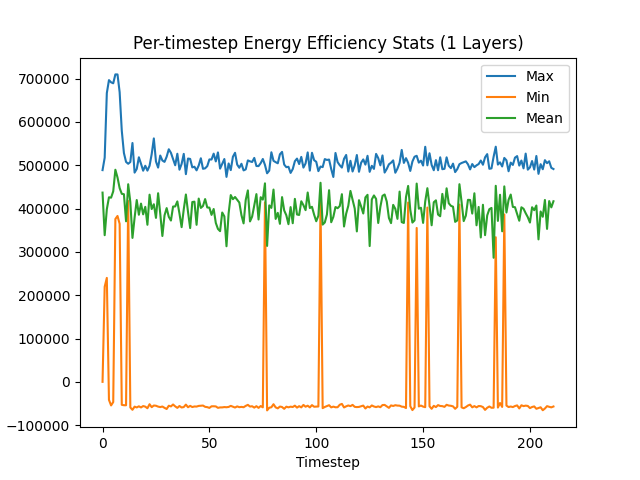
\includegraphics[width=0.42\textwidth]{figures/test9/1_timestep_energy_eff.png}
%       }
%       \hspace{1mm}
%    \subfigure[Energy Efficiency Across 30 Episodes]{\label{fig:ep_energy_eff}
%           %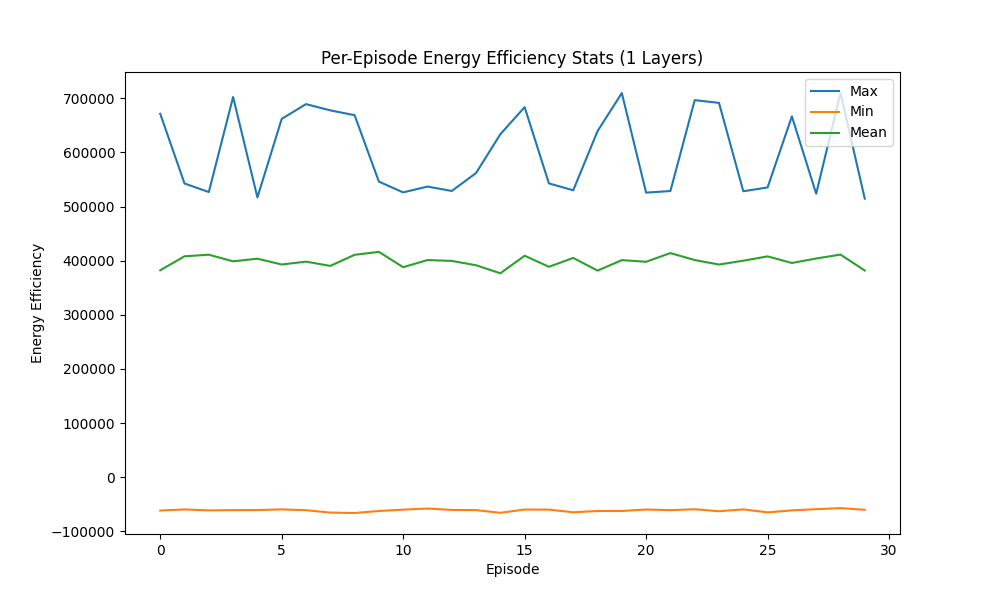
\includegraphics[width=0.45\textwidth]{figures/test9/1_episode_energy_eff.png}
%           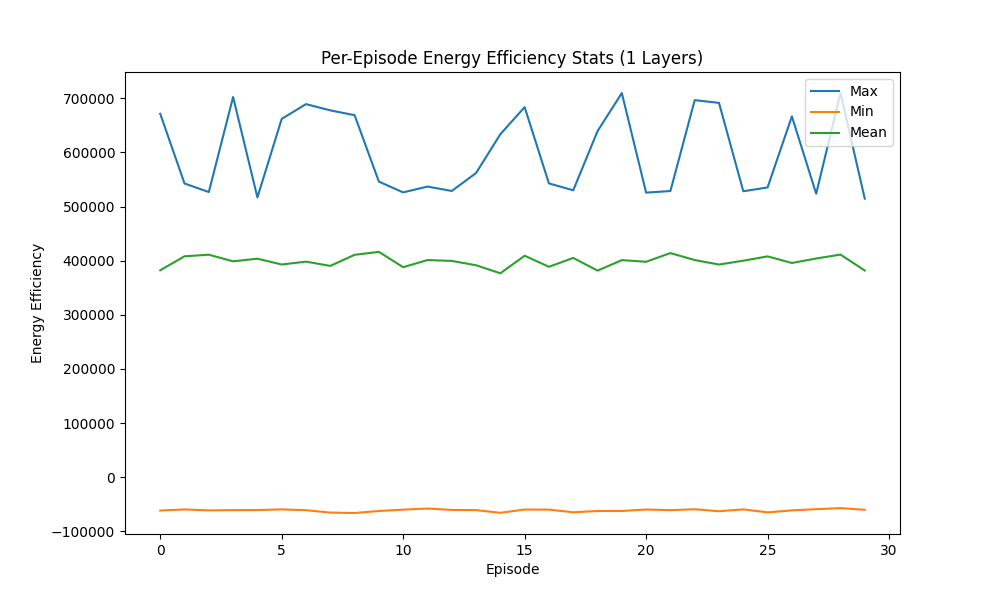
\includegraphics[height=0.2\textheight]{figures/test9/1_episode_energy_eff.png}
%       }
%       \caption{Energy Efficiency Data using a \acrshort{per}}
%       \label{fig:energy_eff_figs}
%\end{figure}
\subsection{Data Exchange Rate}
The data exchange rate $R_{U, k} (t)$ is used to shape the reward allocation along with penalties for violating the constraints of the joint optimisation problem. 
As rewards are dependent on the data exchange and secrecy rates for all \acrshort{lu}s and $\eta (t)$ is a function of $R_{U, k} (t)$, the maximisation of $\eta (T)$ requires that $R_{U, k} (t)$ is maximised and $E_{cons}$ is minimised.

\begin{figure} [ht!]
    \centering
    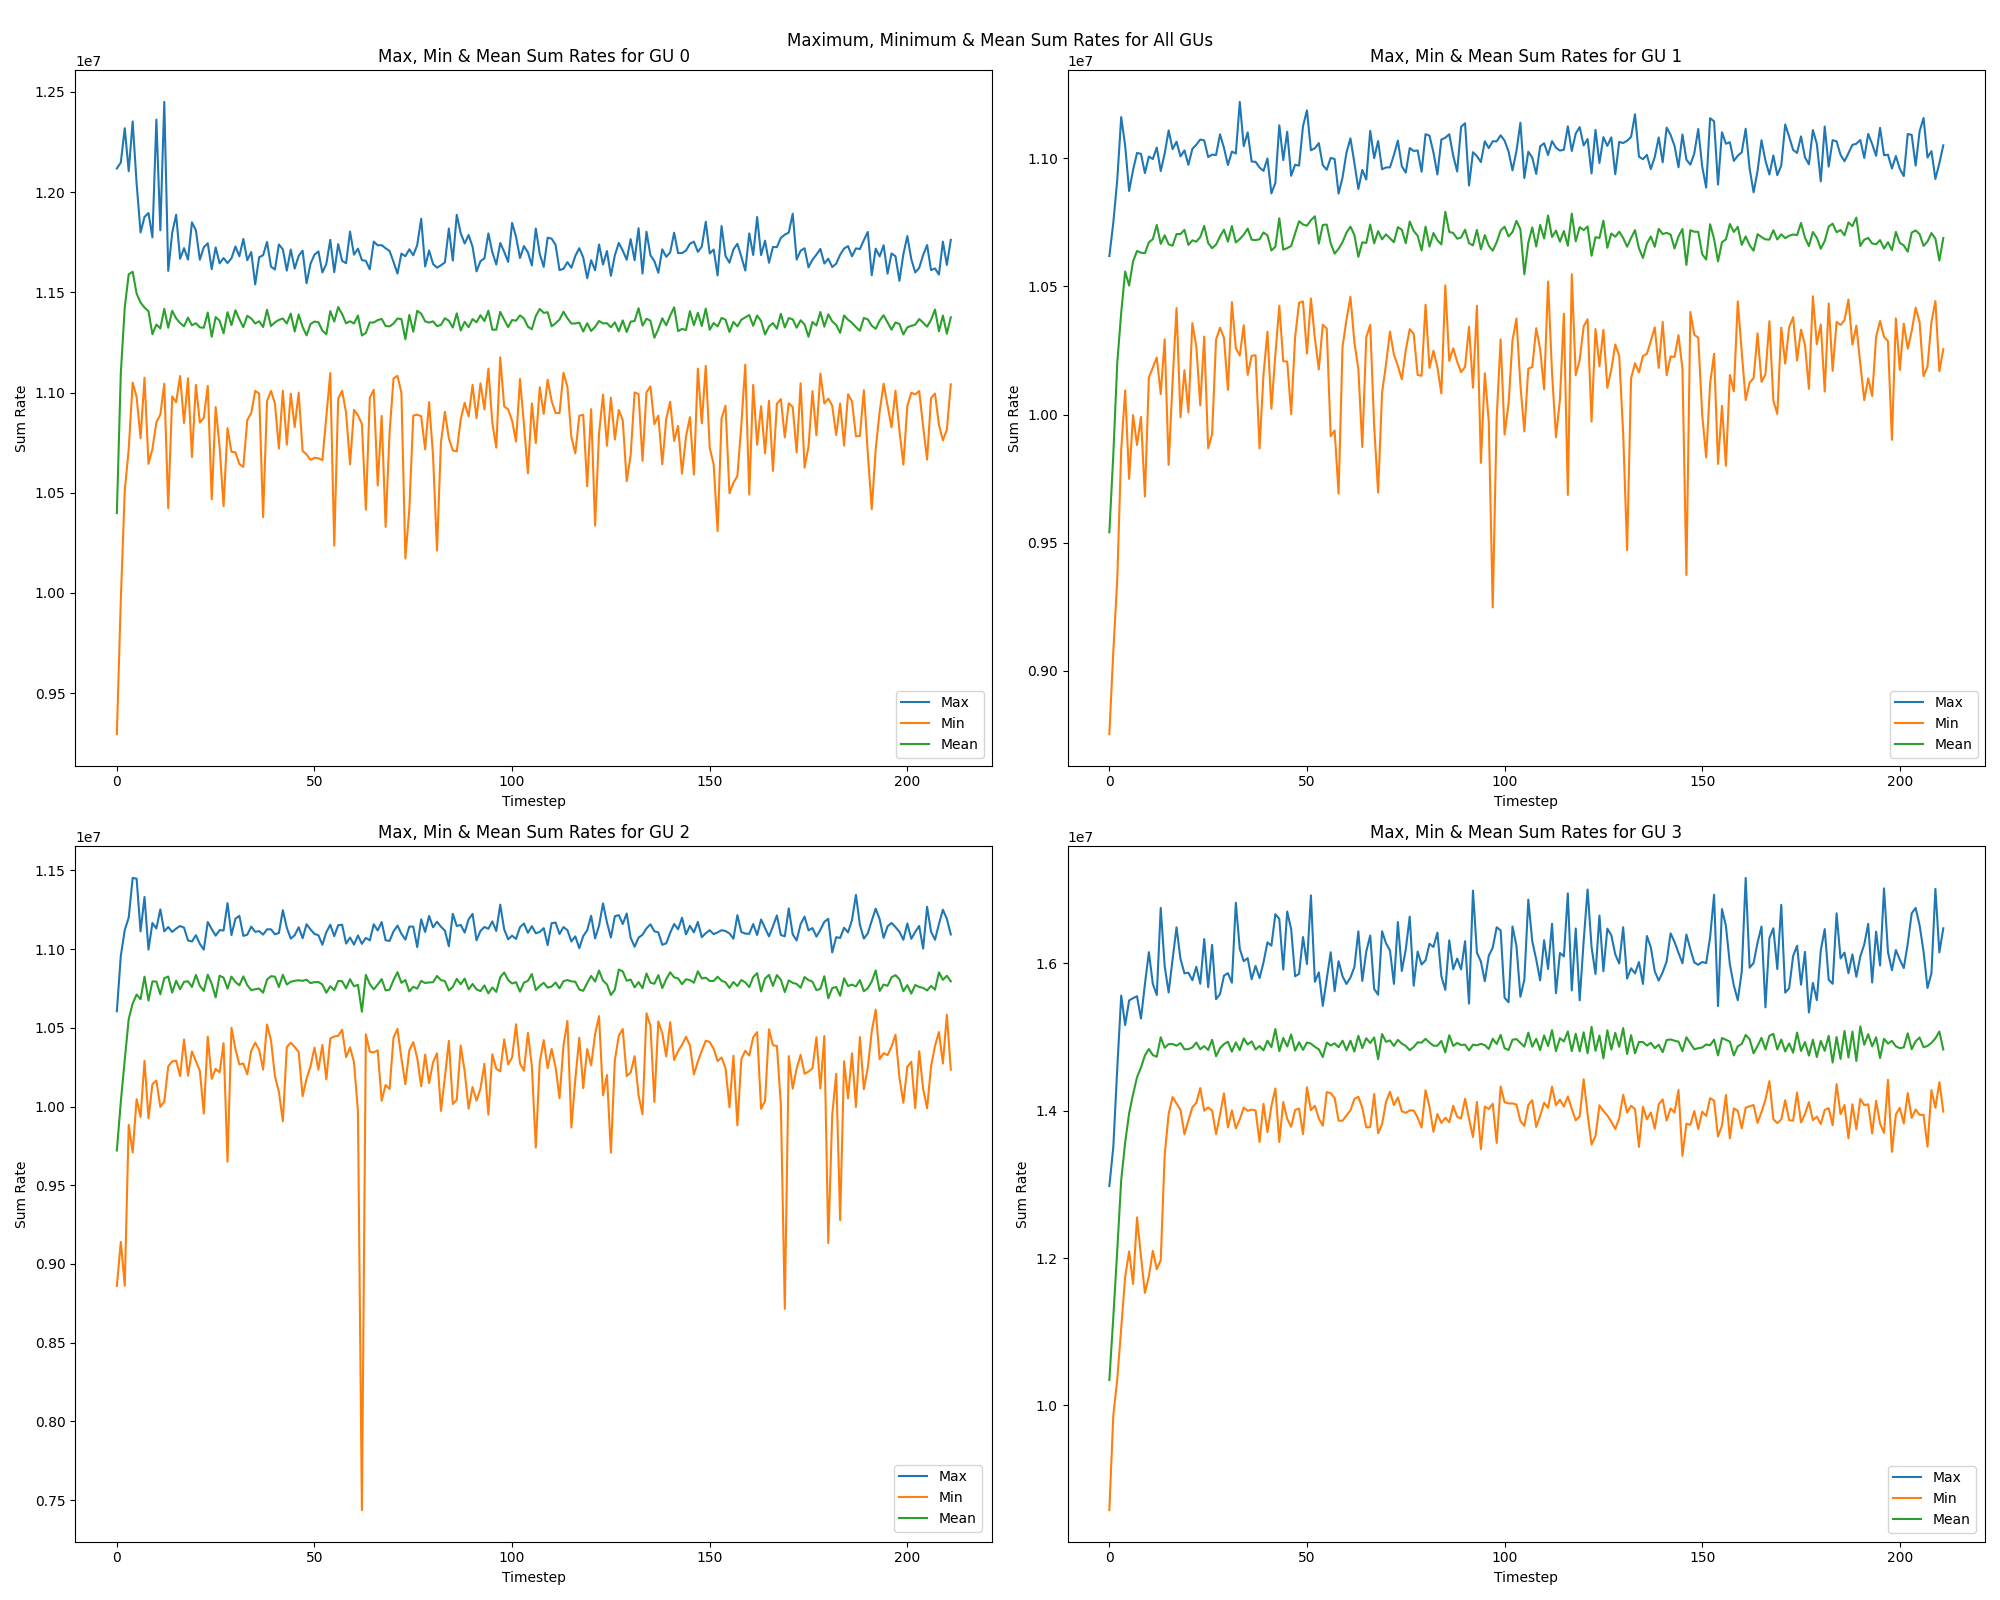
\includegraphics[width=0.9\textwidth]{figures/test9/fixed_1_timestep_sum_rate_all_GUs.png}
    \caption{Maximum, Minimum \& Mean $R_{U, k} (t)$ Values in Mbps from $t$ to $T$ Across 30 Episodes}
    \label{fig:timestep_sum_rates_all_gus}
\end{figure}
As shown in Fig. \ref{fig:timestep_sum_rates_all_gus}, for all of the legitimate \acrshort{gu}s in the simulated scenario, the average sum rate converges from $0$ to above 10 Mbps for $R_{min} = 9.5\ Mbps$ consistently within a short period of time. 

Fig. \ref{fig:episodes_sum_rates_all_gus} displays the maximum, minimum and mean values for the data exchange rates across 30 episodes. 
Again, it can be seen that the agent effectively managed to learn to maximise $R_{U, k} (t)$ for all \acrshort{lu}s such that the $R_{min}$ threshold has been met for all \acrshort{lu}s, ensuring fairness in the distribution of $R_{U, k} (t)$ for all $\mathcal{K}$ \acrshort{lu}s. 
\begin{figure} [ht!]
    \centering
    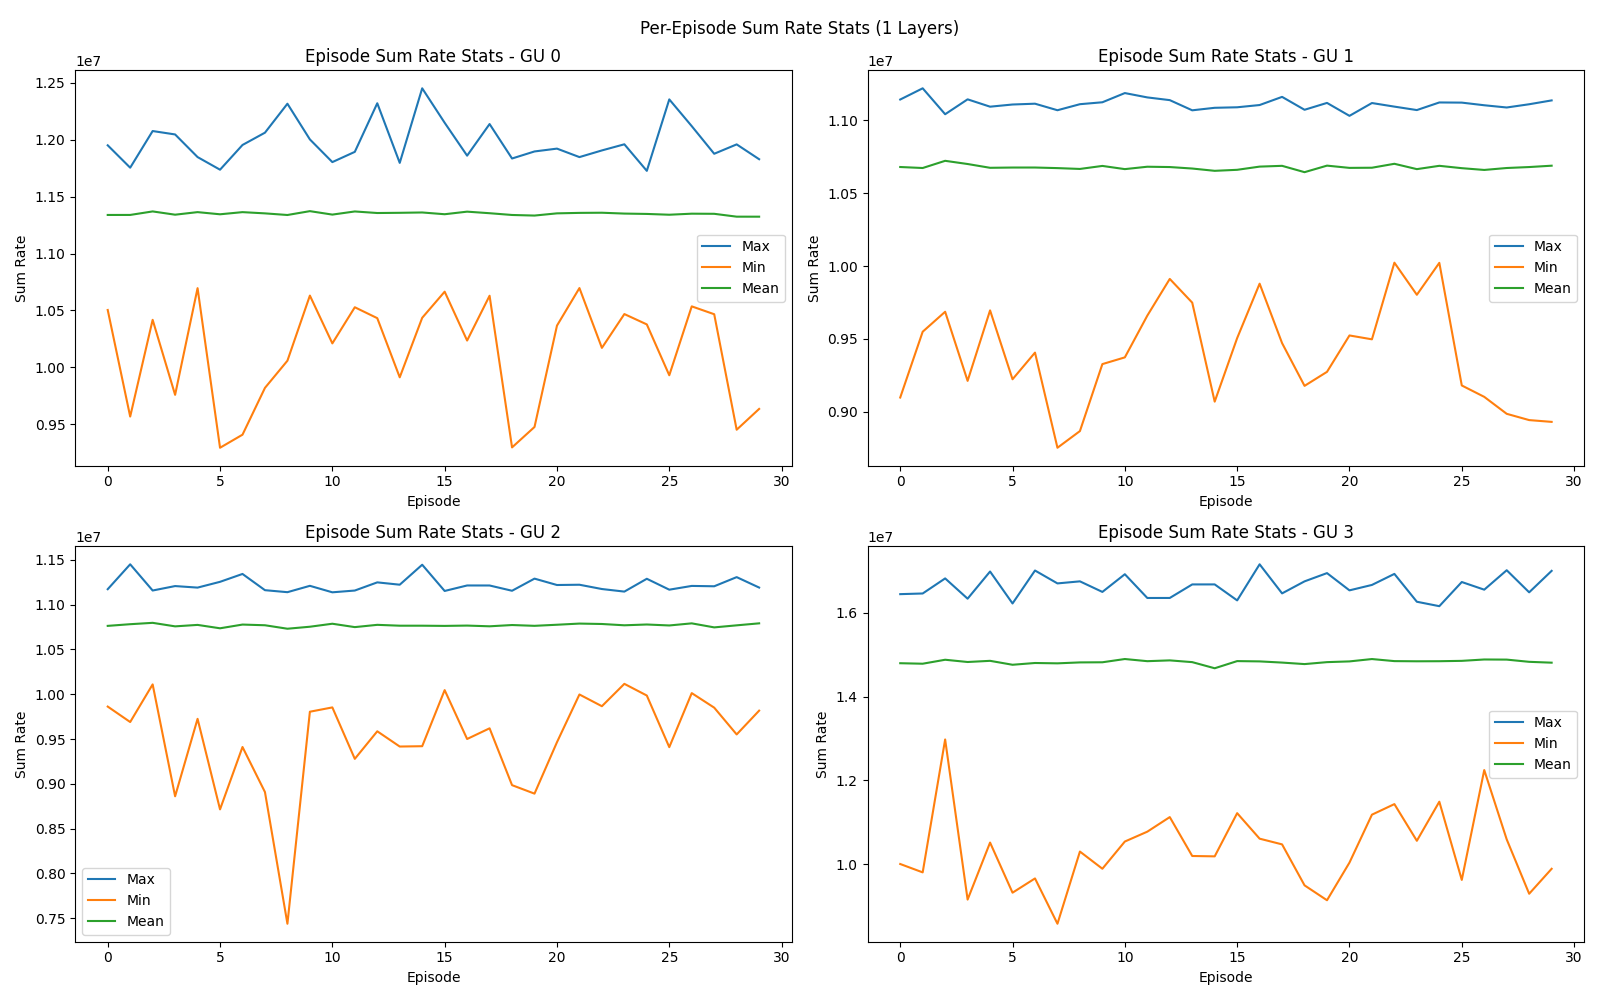
\includegraphics[width=0.9\textwidth]{figures/test9/1_episode_sum_rate_stats.png}
    \caption{Maximum, Minimum \& Mean $R_{U, k} (t)$ in Mbps Values Across 30 Episodes}
    \label{fig:episodes_sum_rates_all_gus}
\end{figure}

This demonstrates that the agent effectively learns to maximise the data exchange rate as well as the fairness in data rates for all \acrshort{gu}s such that all \acrshort{gu}s receive an acceptable and consistent \acrshort{qos}. 
None of the \acrshort{lu}s have a value for $R_{U, k} (t) < R_{min}$ upon convergence, thus adhering to the constraints of the optimisation of $R_{U, k} (t)$. 

%\begin{figure}[ht!]
%    \centering
%    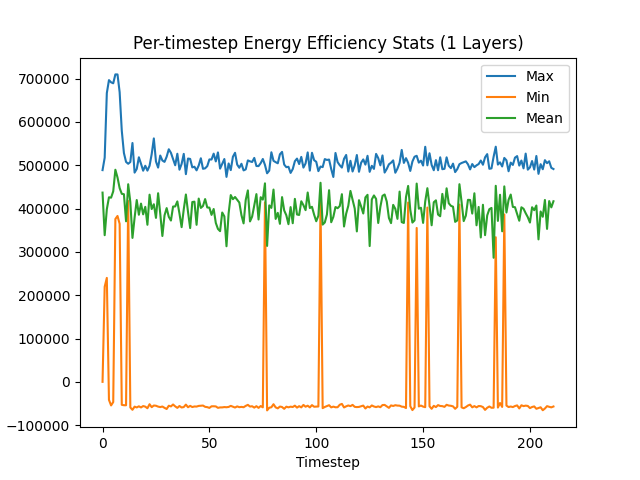
\includegraphics[width=0.5\linewidth]{figures/test9/1_timestep_energy_eff.png}
%    \caption{Caption}
%    \label{fig:step_energy_eff}
%\end{figure}
%
%\begin{figure}[ht!]
%    \centering
%    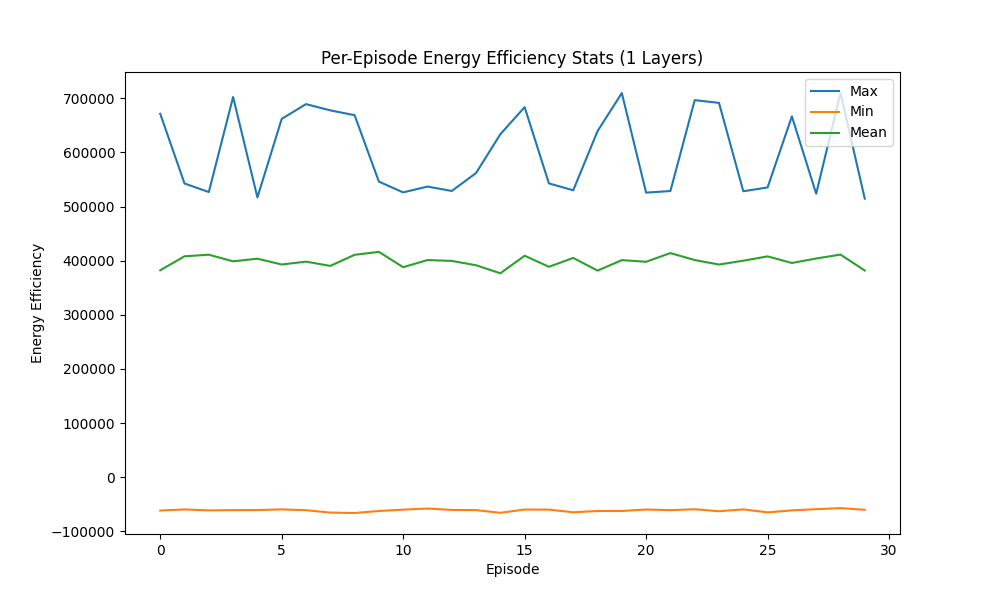
\includegraphics[width=0.5\linewidth]{figures/test9/1_episode_energy_eff.png}
%    \caption{Caption}
%    \label{fig:ep_energy_eff}
%\end{figure}
%\subsection{Data Exchange Rate}

\subsection{Secrecy Rate}
The secrecy rate for the \acrshort{uav}-\acrshort{lu} communications had to be above $R_{min}^{sec} = R_{min} = 9.5\ Mbps$. 
This was achieved with a single layer in the actor-critic quantum circuits and is shown in Fig. \ref{fig:timestep_secrecy_rate_all_gus} and Fig. \ref{fig:episode_secrecy_rate}, respectively. 

\begin{figure} [ht!]
    \centering
    %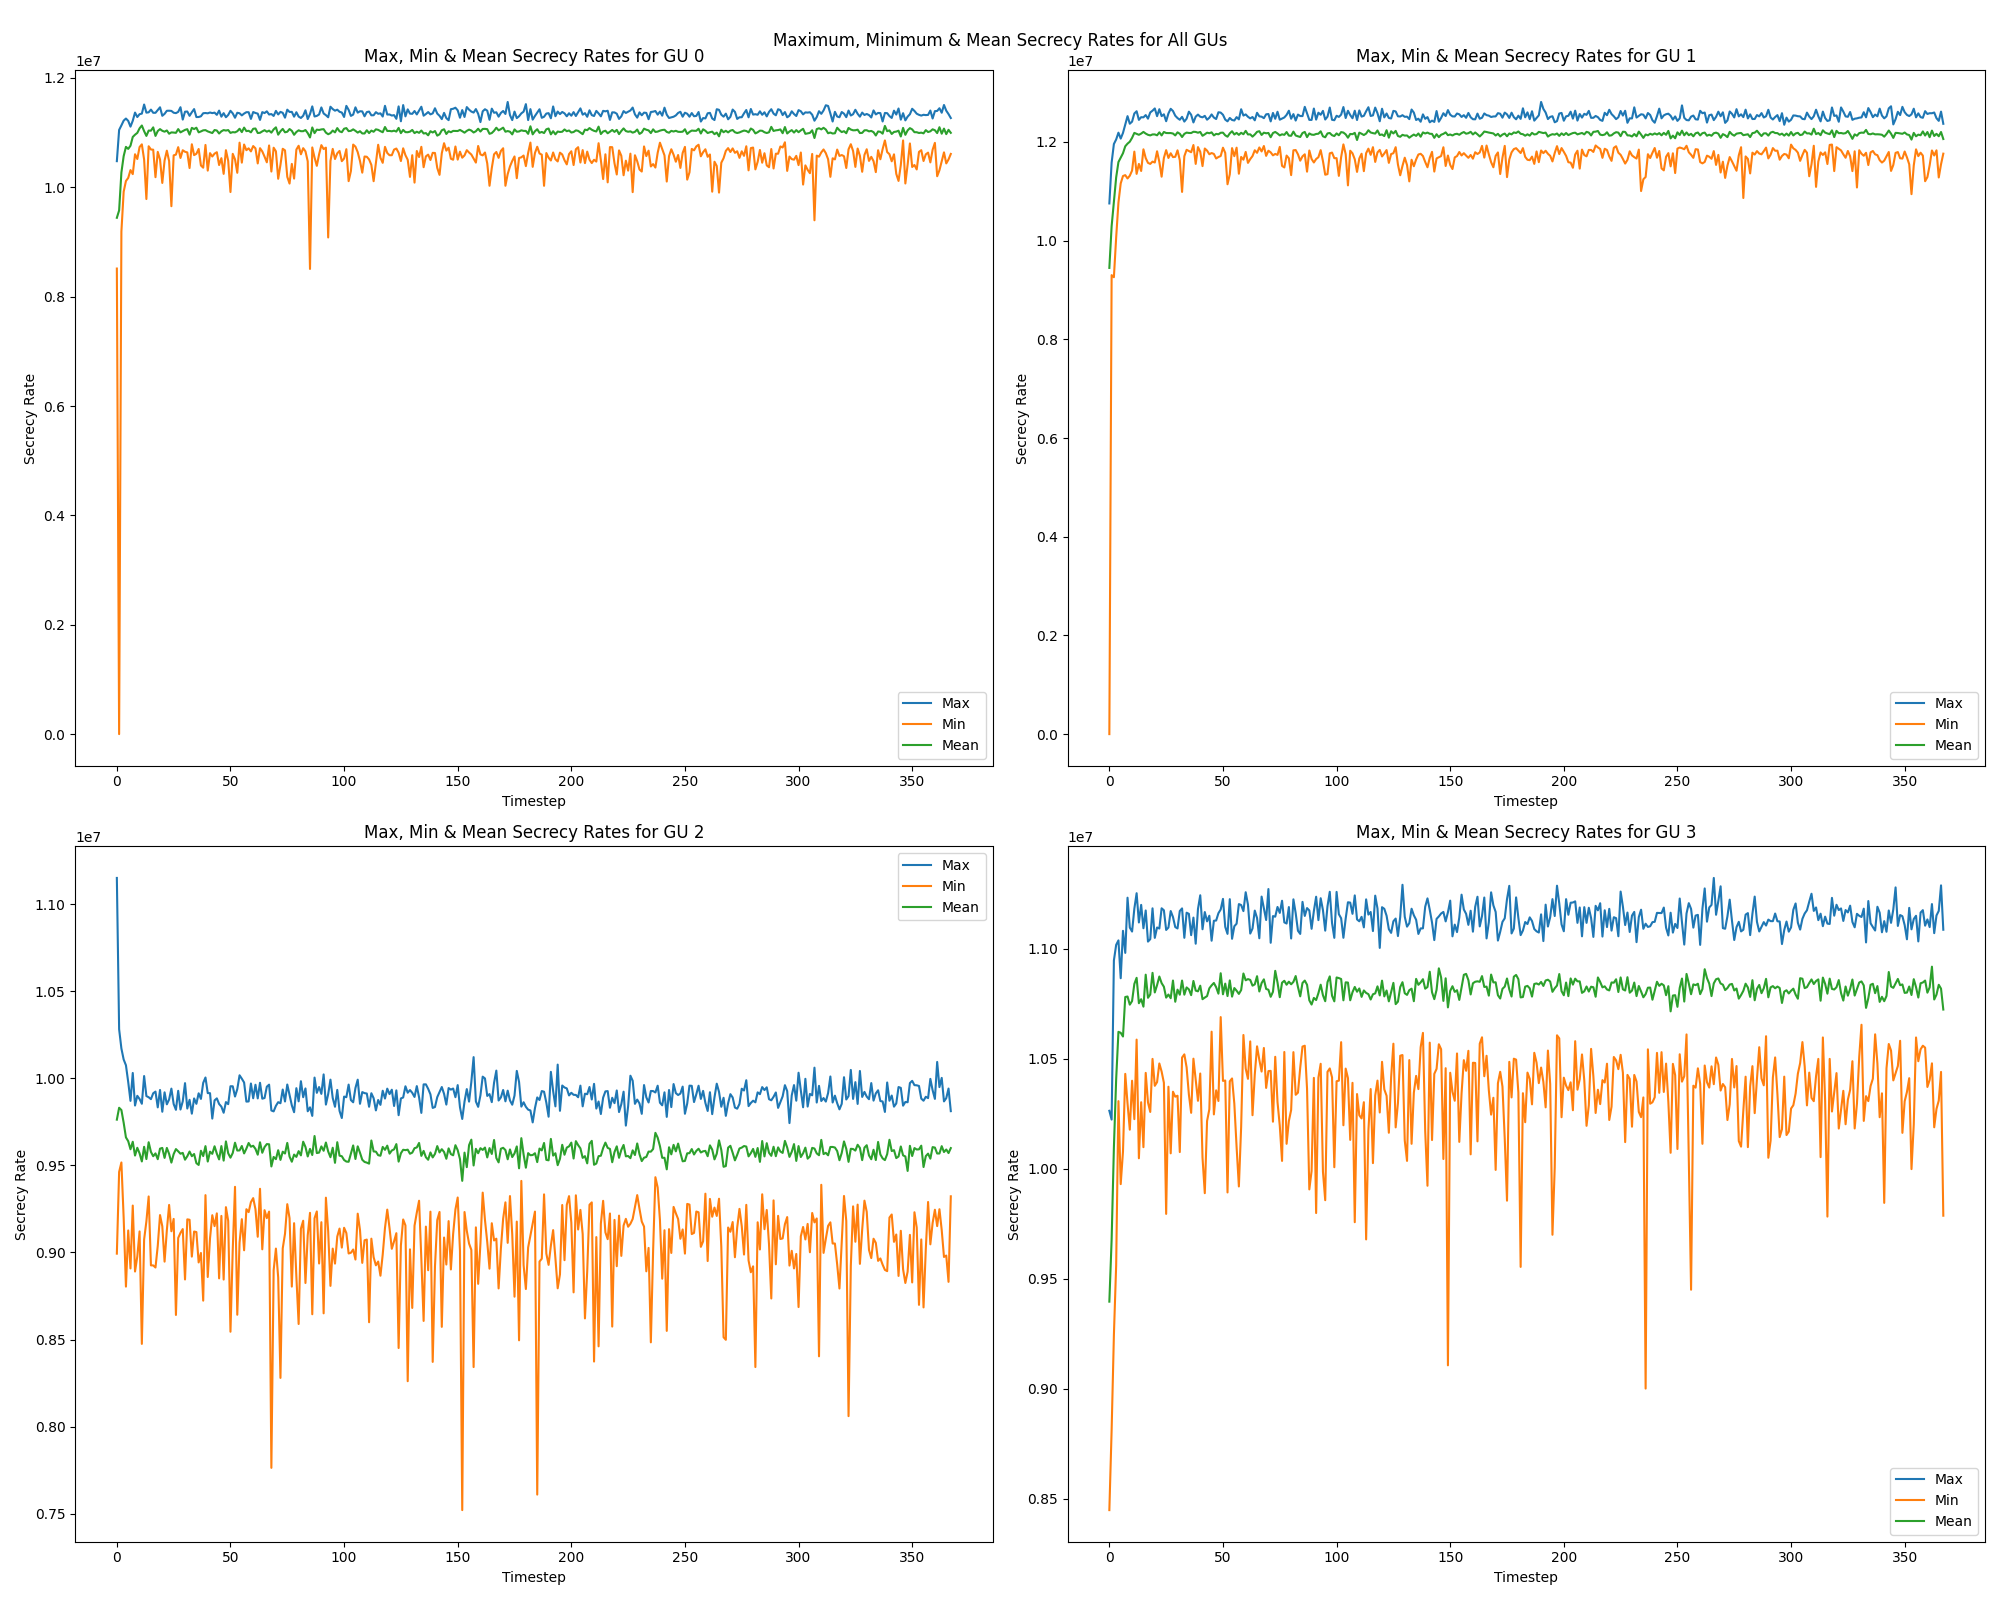
\includegraphics[width=1\textwidth]{figures/eve_test1/1_timestep_secrecy_rate_all_GUs.png}
    %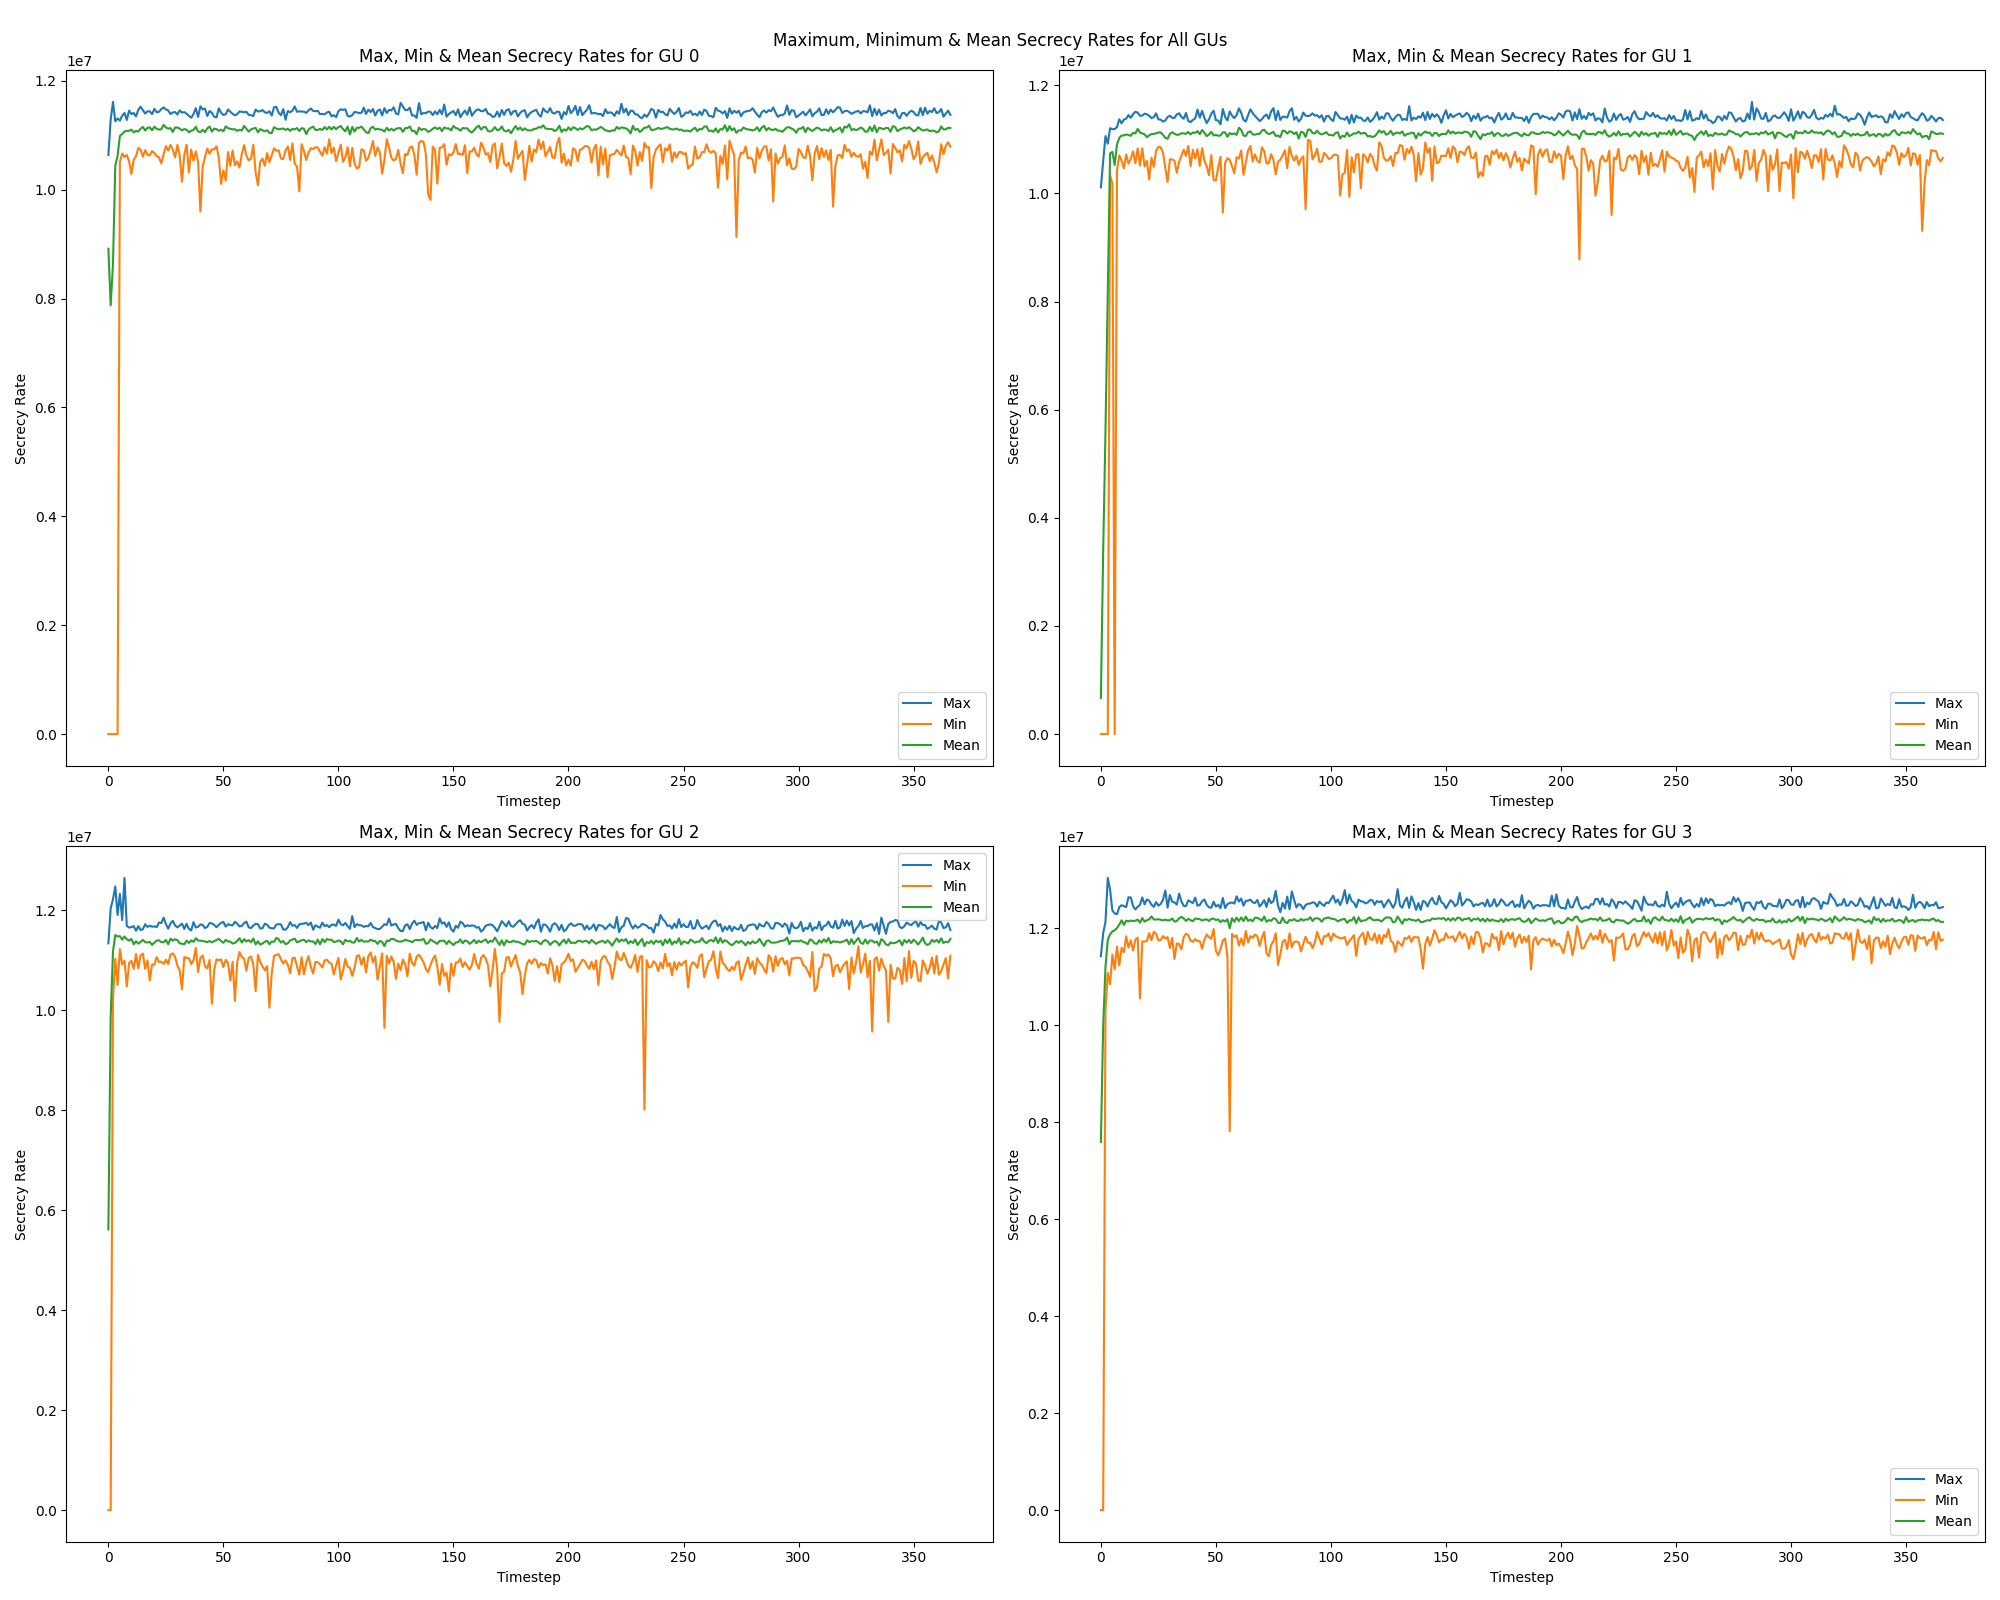
\includegraphics[width=1\textwidth]{figures/eve_out/1_timestep_secrecy_rate_all_GUs.png}
    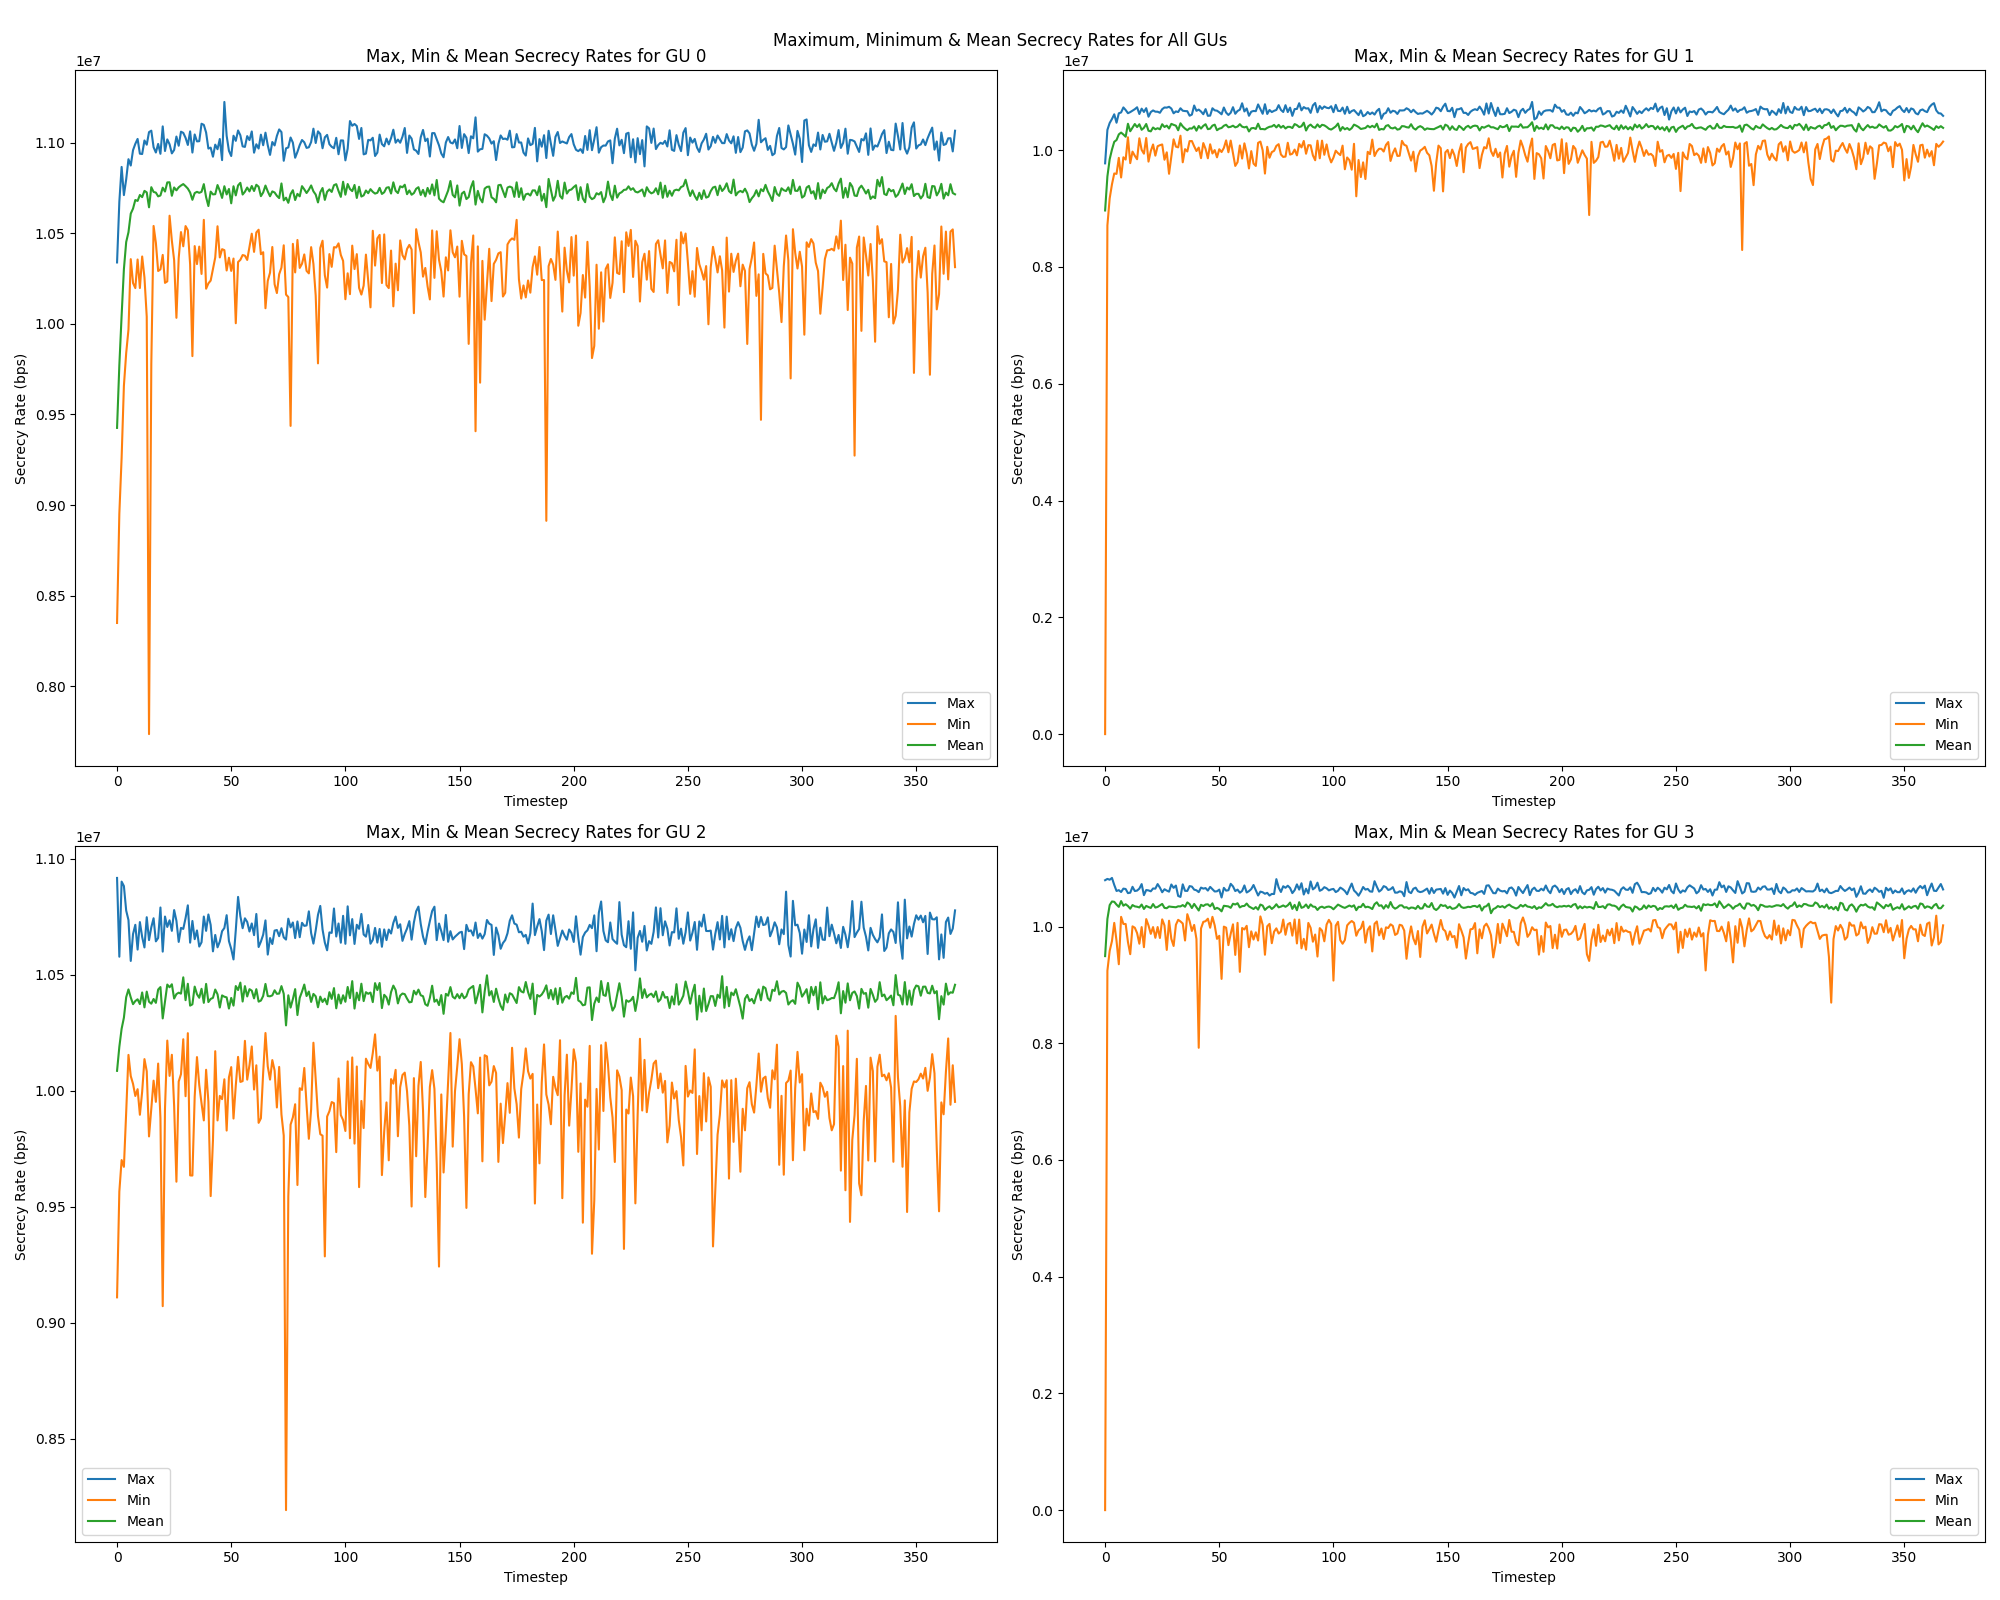
\includegraphics[width=0.9\textwidth]{figures/plots_eve_outputs/test3/1_timestep_secrecy_rate_all_GUs.png}
    \caption{Maximum, Minimum \& Mean Secrecy Rates for all \acrshort{lu}s for each Timestep Across 30 Episodes}
    \label{fig:timestep_secrecy_rate_all_gus}
\end{figure}

\begin{figure} [ht!]
    \centering
    %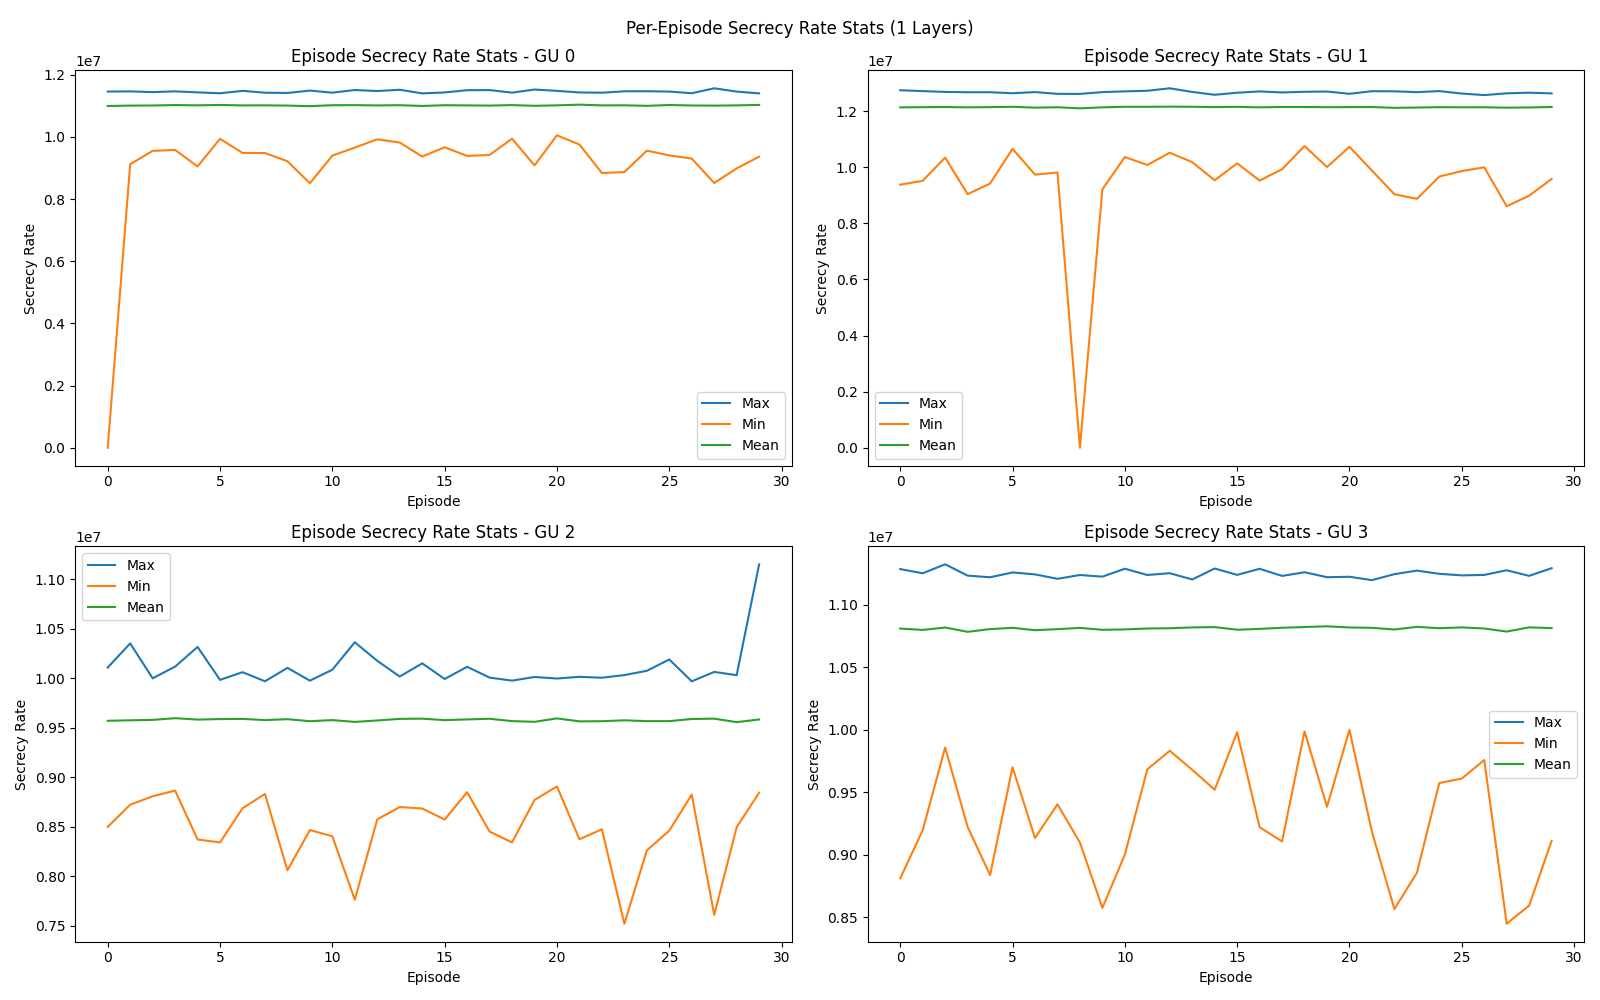
\includegraphics[width=1\textwidth]{figures/eve_test1/1_episode_secrecy_rate_stats.png}
    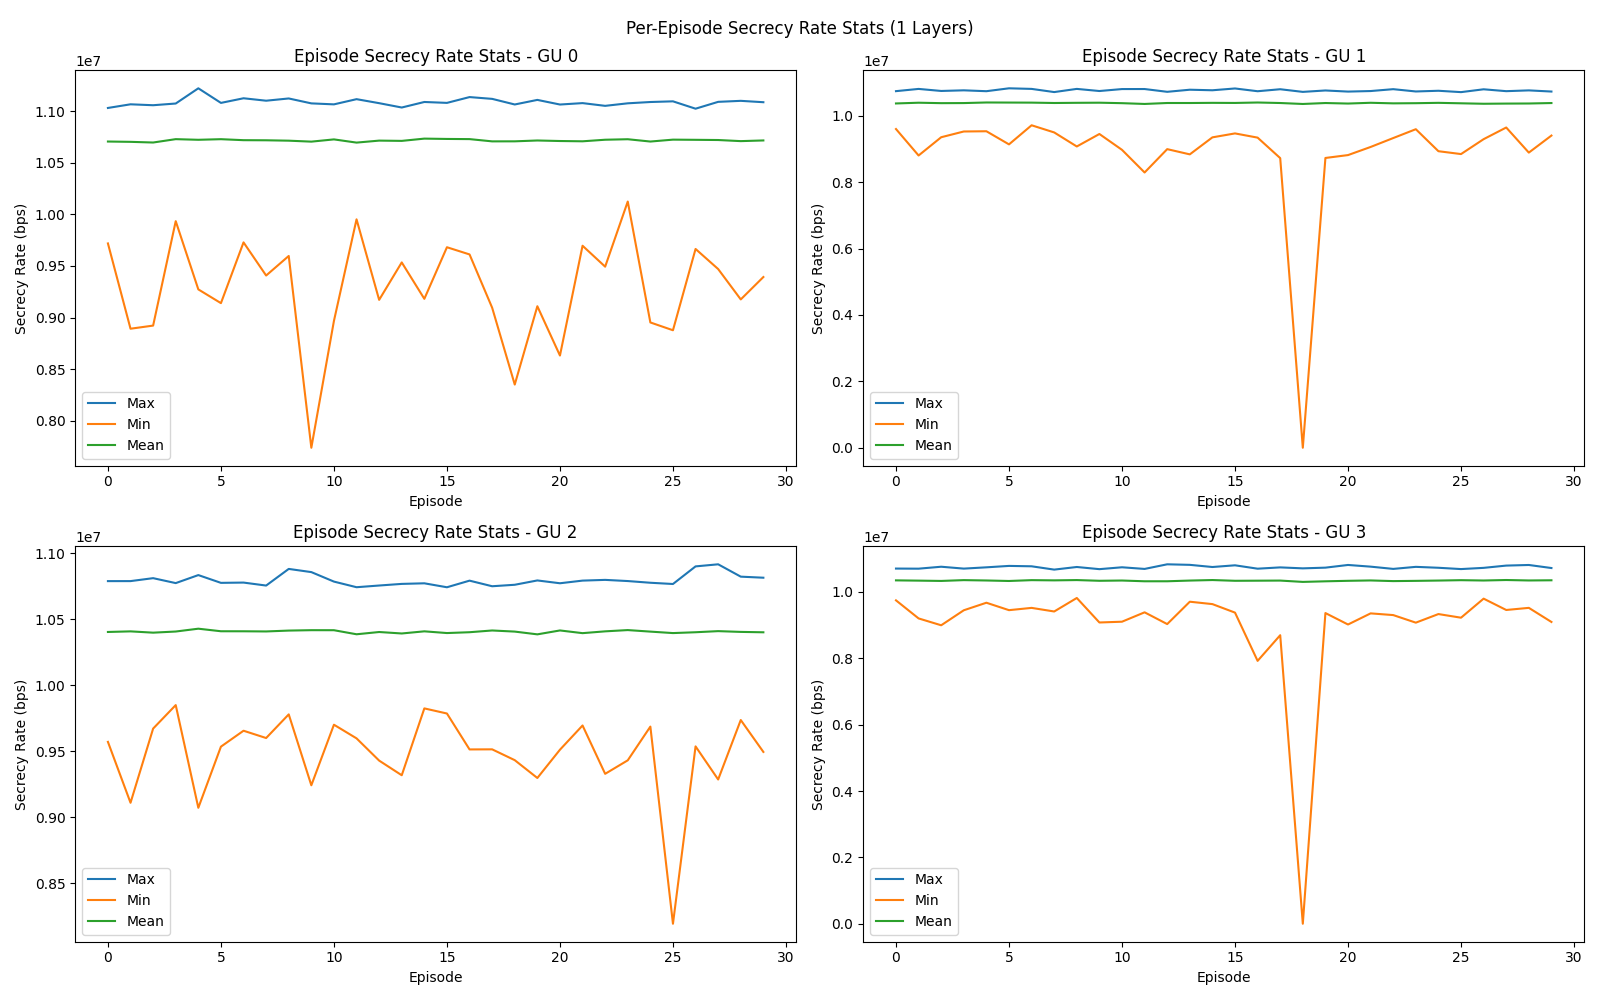
\includegraphics[width=0.9\textwidth]{figures/plots_eve_outputs/test3/1_episode_secrecy_rate_stats.png}
    \caption{Maximum, Minimum \& Mean Secrecy Rates for all \acrshort{lu}s Across 30 Episodes}
    \label{fig:episode_secrecy_rate}
\end{figure}

It can be seen that $R_{U, k}^{sec}$ converges to above $R_{min}^{sec}$ consistently, which is in-line with the increase in $R_{U, k}$, as the increase in $R_{U, k}^{sec}$ is dependent on the increase of $R_{U, k}$.
As shown in Fig. \ref{fig:timestep_secrecy_rate_all_gus} and Fig. \ref{fig:episode_secrecy_rate}, the threshold for the minimum acceptable secrecy rate was reached for all of the legitimate \acrshort{gu}s. 
No single \acrshort{lu} was left for it's average total secrecy rate $\bar{R}_{U, k}^{sec}$ to fall below $R_{min}^{sec}$. 

Each \acrshort{lu} had its secrecy rate converge to above 10 Mbps within the simulation to the point of the secrecy rate converging onto the value of the data exchange rate. 
This is a desirable outcome for this problem, demonstrating the efficacy of spiking the \acrshort{uav}-\acrshort{lu} communications with an \acrshort{ans}. 
This demonstrates that the Eve links were so affected by the \acrshort{ans} that their \acrshort{snr} plummeted to a very low value, i.e., any form of useful information from the signal was overpowered entirely by the \acrshort{ans}. 
This shows that the eavesdropping rate has dropped, increasing the secrecy rate and minimised the capabilities for Eves to conduct \acrshort{mitm} attacks on the \acrshort{lu}s. 
\section{\texorpdfstring{\acrshort{drl}}{DRL} Performance}
%\hl{DETAIL \& PLOT DRL ALGORITHM PERFORMANCE WITH DRL METRICS}
\subsection{Local Loss}
The critic loss within the algorithm began to decrease and stabilise around a small set of values for a single layer, as shown in \ref{fig:single_layer_critic_loss}. 

\begin{figure}[ht!]
    \centering
    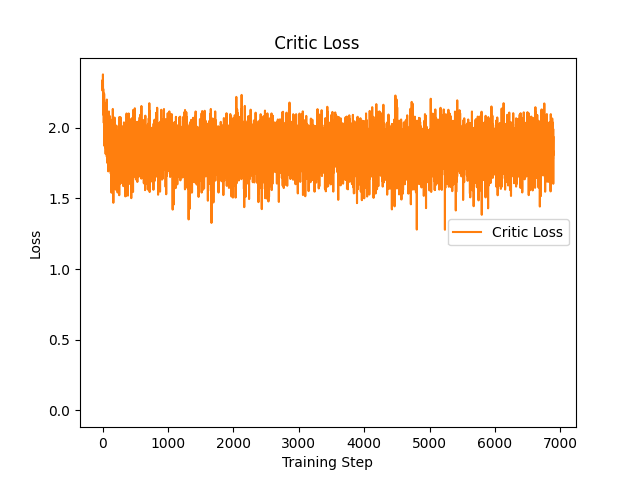
\includegraphics[width=0.75\linewidth]{figures/test9/1_layers_losses.png}
    \caption{Critic Loss for M = 1}
    \label{fig:single_layer_critic_loss}
\end{figure}
The results for the loss function from the critic network are quite noisy as a result of having to sampling and decode the values $K_{shot}$ times in a simulated open quantum system. 
The length of the quantum circuit is also quite large, with 17 inputs being fed into the critic network, leading to a noisy output prior to decoding, however, this did not appear to impact the results presented in the previous section in a negative way. 
\section{Quantum Actor-Critic Network}
The actor-critic network quantum circuitry appeared to perform most optimally with a single layer within the ansatz rather than increasing the number of layers. 

The quantum actor-critic network was tested with 1-5 layers within the system. 
This was performed to determine the impact on the number of layers and if the increase in the number of layers positively or negatively impacted the performance of the system beyond a particular number of layers. 

\subsection{Impact of the Number of Layers on Performance}
It was found that for higher numbers of layers beyond a single layer within the ansatz that the performance of the \acrshort{lqdrl} algorithm began to degrade and become far more unpredictable, leading to very noisy curves for the \acrshort{uav} trajectory, $\eta_{EE} (t)$, $R_{U, k}$ and $R_{U, k}^{sec}$. 

After 3 layers within the actor-critic ansatz circuits, it was observed that the results for the secrecy rate, data exchange rate, trajectory and energy efficiency all became far too noisy and unpredictable to be of any practical value. 

This phenomenon may arise from the fact that the same values are being recomputed repeatedly despite only a single layer being useful, leading to increased levels of noise arising from the increased depth of the quantum circuits. 

Figures with data for each timestep of each episode for each number of layers can be found in \ref{appendix_layers_figures}. 

As shown in \ref{appendix_layers_figures}, the results are consistent and converge towards their optimal values for the \acrshort{uav} trajectory and the data exchange rate, however, for increasing numbers of layers, the \acrshort{uav} can either do the opposite of what its objective is for M = 2 and begins to become too noisy and unpredictable for 3-5 layers. 
In the case of M = 2, the fact that the data exchange rate and the distance between the \acrshort{uav}-\acrshort{bs} and the \acrshort{lu} centroid converged to the opposite of the desired outcome could be useful for providing some insights into the optimisation problem, e.g., it could serve as a means to model a dual optimisation problem, however, this has not been explored extensively as part of this thesis. 